Wenn die Einwirkungen aus Erdbeben sehr hoch werden, zum Beispiel durch eine hohe Anforderung an den Bedeutungsbeiwert oder sich das Bauwerk in einem Starkbebengebiet befindet, ist es meistens technisch und wirtschaftlich günstiger, die Struktur von der Einwirkung zu isolieren, damit sie dieser nicht mehr vollends ausgesetzt wird.

Es können leichtere Konstruktionen gebaut werden, die durch geringere Aufwendung an Material die Kosten senken und die Nachhaltigkeit durch senken des Ausstoßes an CO\textsubscript{2} erhöhen.

Die horizontale Isolation ist keine Lösung der Neuzeit. Schon die Baumeister im alten China ordneten zwischen Fundament und Grundplatte eine Schicht aus rolligem Sand an \cite{Taylor}.
Im zwanzigsten Jahrhundert folgten einige Patente mit dem selben Grundprinzip und 1921 realisierte Frank Lloyd Wright das Imperial Hotel in Tokyo mit einer Isolation mittels einer Schicht 3m mächtigen aus Weichboden. Das Gebäude überstand ein 2 Jahre später aufgetretenes schweres Erdbeben nahezu unbeschadet \cite{Reitherman}.

Für die Isolierung stehen einige verschiedene Mechanismen, wie zum Beispiel kinematische Lager, Gleitpendelisolatoren und Elastomerlager (ggf. mit Bleikern) zur verfügung.
In dieser Arbeit sollen nur Gleitpendelisolatoren betrachtet werden.


\section{Gleitpendelisolatoren}
\label{sec:gleitisolatoren}

 Gleitpendelisolatoren bestehen aus zwei spherisch angeformten Lagerplatten zwischen denen ein Gleitschuh geschaltet wird.

\begin{figure}[H]
    \centering
    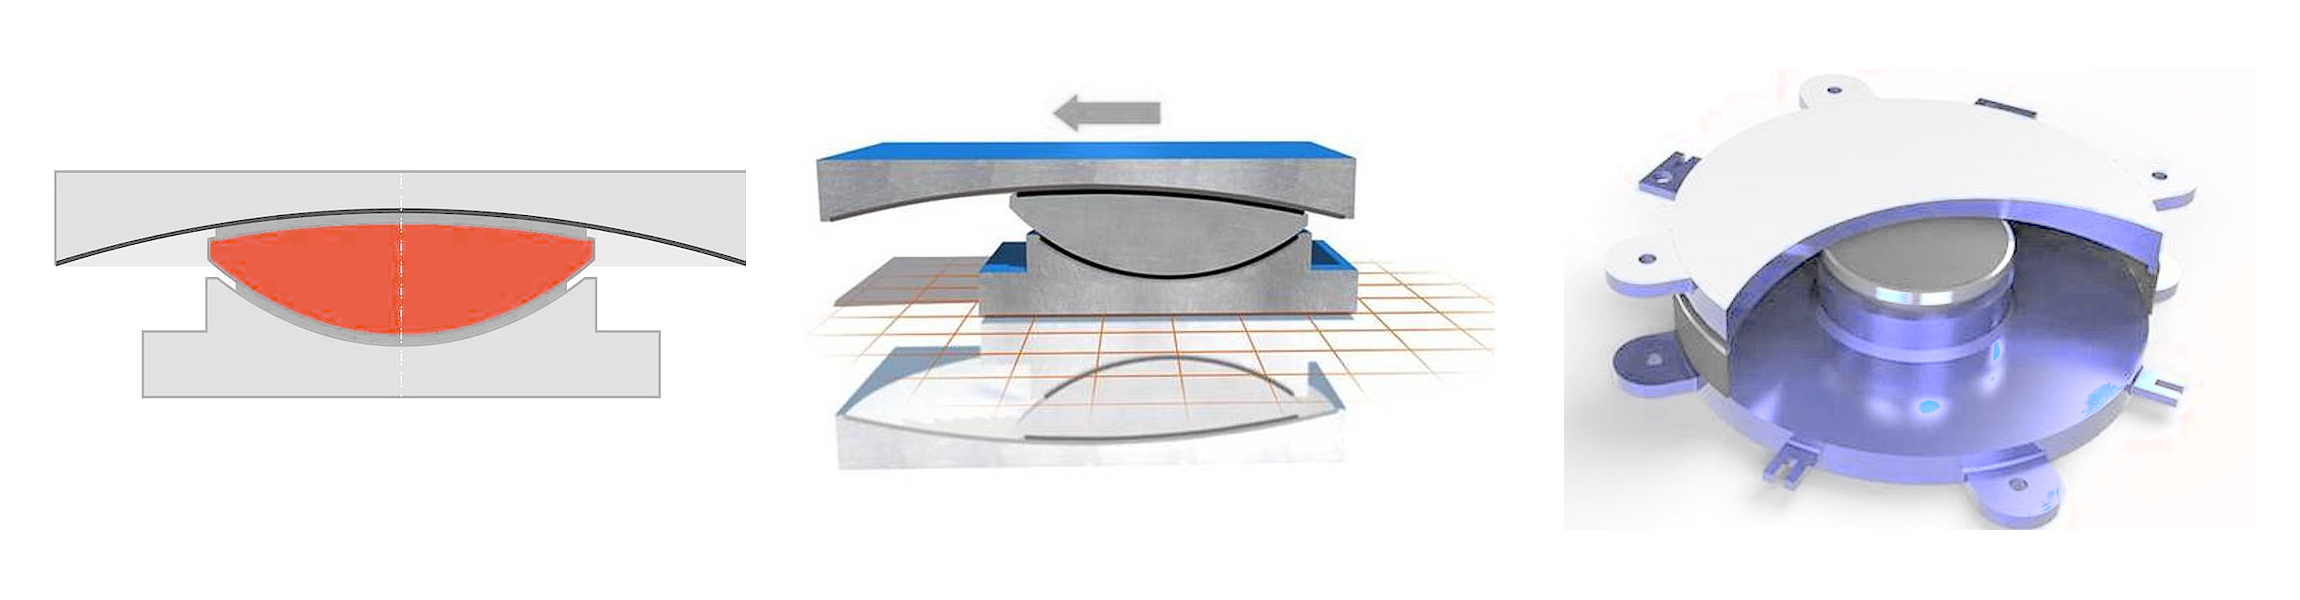
\includegraphics[width=0.9\textwidth]{maurer.png}
    \caption{Gleitpendelisolator [Maurer SE (maurer.eu)]}
\end{figure}

Die Reibung zwischen den Schnittstellen und somit die Energiedissipation kann eingestellt werden.
Bei einem zu hohen Reibkoeffizienten besteht jedoch die Gefahr, dass die Rückzentrierung nicht mehr gewährleistet werden kann, welche ein großer Vorteil der Gleitpendelisolatoren ist.
Zur Erhöhung der Dissipation können aber auch zusätzliche viskose Dämpfungselemente angeordnet werden (\cref{Dampener}).

\begin{figure}[h]
    \centering
    \subfloat[Gleitpendelisolator]{{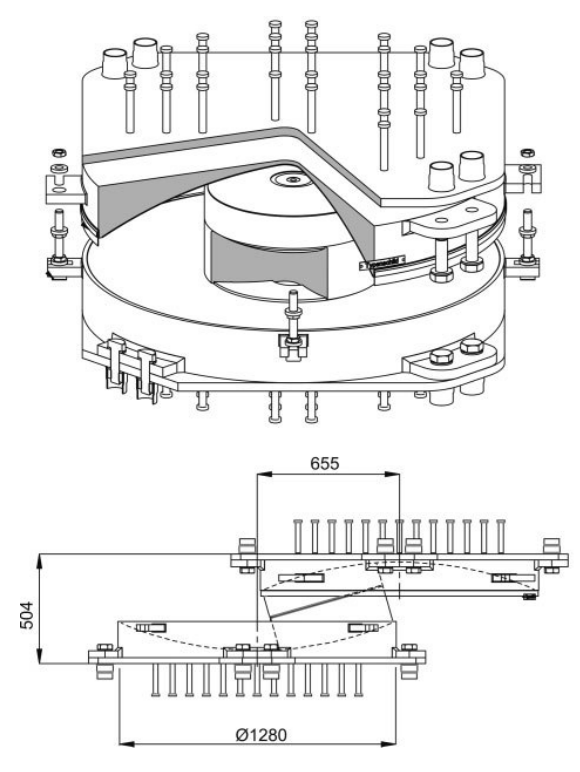
\includegraphics[width=0.45\linewidth]{Algerien_1.png} }}%
    \qquad
    \subfloat[Viskoser Hydraulikdämpfer]{{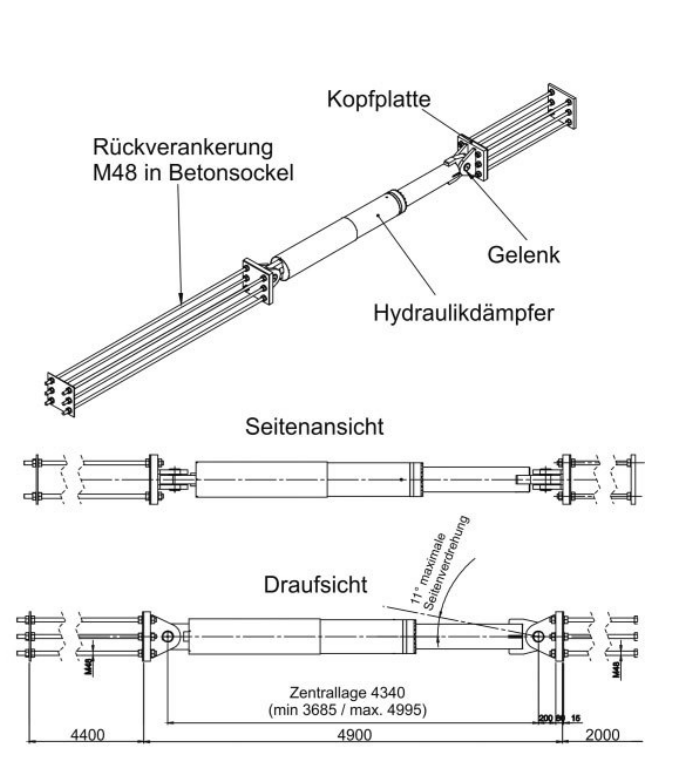
\includegraphics[width=0.45\linewidth]{Algerien_2.png} }}%
    \caption{Bauform der Iolatoren (a) und Dämpfer (b) der Großen Moschee von Algerien \cite{AKK}}%
\end{figure}

\begin{figure}[h]
    \centering
    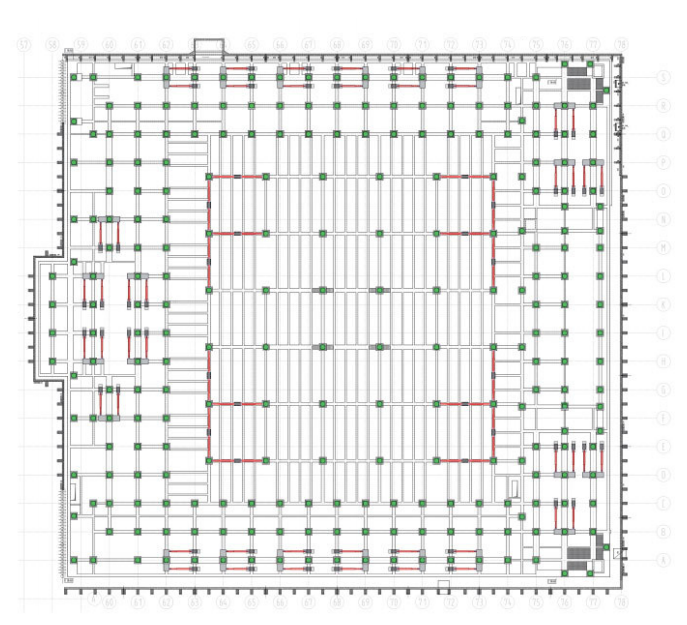
\includegraphics[width=0.9\textwidth]{Algerien_3.png}
    \caption{Verteilung der Iolatoren (grün) und Dämpfer (rot) im Grundriss \cite{AKK}}
	\label{Dampener}
\end{figure}

\pagebreak

\section{Funktionsweise}
\label{sec:funktion}

Isolatoren stellen eine Ebene zwischen der Gründung und dem aufgehendem Bauwerk dar. Sie haben eine deutlich geringere Steifigkeit als die zu isolierende Struktur, wodurch zwar große Verschiebungen am Isolator auftreten (\cref{Verteilung}), aber die Grundschwingzeit reduziert wird.
Die relativen Verschiebungen der Struktur werden verringert und somit die Beschleunigungen und ebenso die Trägheitskräfte der Massen reduziert.

\begin{figure}[h]
    \centering
    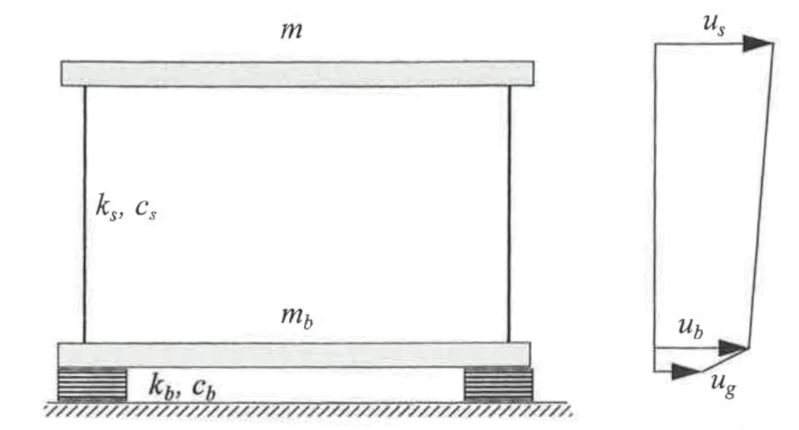
\includegraphics[width=0.9\textwidth]{Verschiebung_iso.png}
    \caption{Verteilung der Verschiebungen an einem isolierten System \cite{Kelly}}
	\label{Verteilung}
\end{figure}

Die Dissipationsfähigkeit, Steifigkeit und Eigenfrequenz dieser Isolatoren kann über den Reibkoeffizienten, den Radius des Pendels und der Masse über dem Isolator beeinflusst werden.

\subsection{Abstimmung}
\label{sec:abstimmung}

Damit der Isolator möglichst effektiv wirkt sollte das Ziel sein die Masse direkt über dem Isolator möglichst groß zur wählen und die Steifigkeit zu reduzieren wobei die aufgehende Struktur möglichst steif sein sollte.
Dadurch sollte die Periode des Isolators $T_I$ möglichst weit von der Periode der Struktur $T_S$ entfernt sein.
Ein Wert, der sich in der Praxis bewährt hat angestrebt zu werden ist $S_I \approx 3 \cdot T_S$.

\subsection{Steifigkeit}
\label{sec:steifigkeit}

Die effektive Steifigkeit kann über die Rückstell- und Reibkraft des Gleitpendellagers berechnet werden. Die Rückstellkraft wird durch die Anhebung der Vertikalkraft (Eigengewicht des Bauwerks) ausgelöst. \cite{Pocanschi}

\begin{figure}[H]
    \centering
    \includegraphics[width=0.9\textwidth]{Pendellager.png}
    \caption{Schematischer Aufbau des Gleitpendellagers im zentriertem sowie im ausgelenkten Zustand \cite{Romen}}
\end{figure}

\begin{align*}
F_{\text{Rück}} &= \frac{G D}{R \cos \theta}\\
F_{\text{Reib}} &= \mu G
\end{align*}

\makebox[0.8cm]{$G$}  Vertikalkraft (Eigengewicht)\par
\makebox[0.8cm]{$D$}  Auslenkung\par
\makebox[0.8cm]{$R$}  Radius der Isolator-Gleitfläche\par
\makebox[0.8cm]{$\theta$}  Winkel der Auslenkung\par
\makebox[0.8cm]{$\mu$}  Reibungskoeffizient des Isolators\par

Für kleine Winkel mit $\cos \theta = 1$ ergibt sich die Steifigkeit zu:

\begin{align}
k_{eff} &= \frac{F_{\text{Rück}} + F_{\text{Reib}}}{D}\nonumber\\
        &= \frac{G}{R} + \mu \frac{G}{D}\label{keff}
\end{align}

\subsection{Dämpfung}
\label{sec:daempdung}

Die effektive Dämpfung ergibt sich aus der Fläche der Hystereseschleife und der effektiven Steifigkeit des Gleitpendellagers. \cite{Huber}\cite{Pocanschi}

\begin{figure}[h]
    \centering
    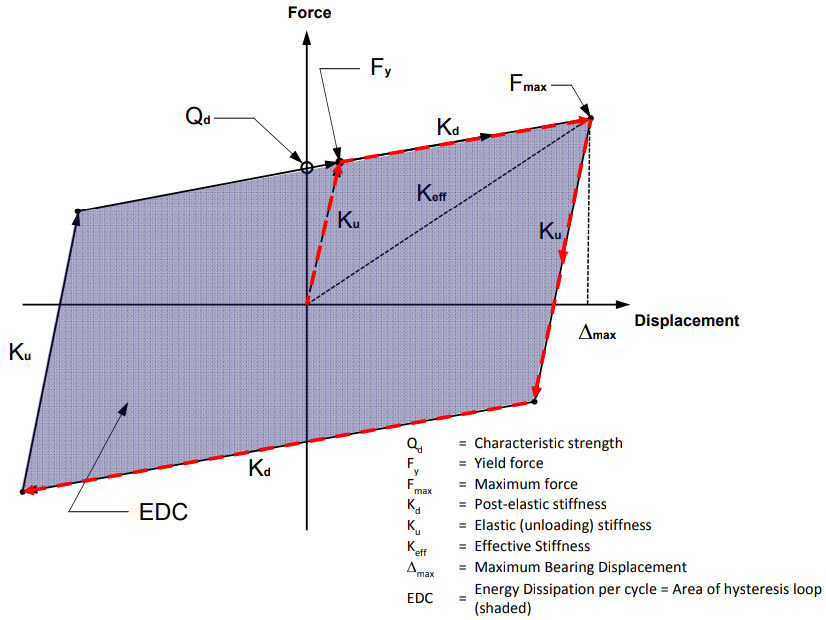
\includegraphics[width=0.9\textwidth]{Hysteresis.png}
    \caption{Hysterese-Zyklus [HDR Engineering Inc.]}
\end{figure}

\begin{align}
\xi_{eff} &= \frac{4 \mu G D}{2 \pi k_{eff} D^2}\nonumber\\
          &= \frac{2}{\pi} \frac{\mu R}{(D + \mu R)}\label{xieff}
\end{align}



\pagebreak

\section{Schwierigkeiten bei der Vordimensionierung}
\label{sec:schwierigkeitenvordimensionierung}

Für eine genaue Berechnung ist es sinnvoll ein Gebäudemodell samt Isolator zu erstellen und mit dem Zeitschrittverfahren und Erdbebenzeitverläufen zu berechnen. Dies ist jedoch sehr aufwendig und bei einer Vordimensionierung nicht immer praktikabel, da sich Parameter noch ändern können.
Ein Ansatz ist es unter der Annahme, dass die Steifigkeit der Struktur sehr hoch ist und die des Isolators $k_I$ die Eigenform dominiert die Gesamtstruktur auf einen Einmassenschwinger mit der effektiven Masse aus Strutkur ($m_S$) und Isolator ($m_I$) zu vereinfachen \cite{Kelly}.
Die Eigenfrequenz kann dann mit

\begin{equation}
\omega = \sqrt{\frac{k_I}{m_S + m_I}}
\end{equation}

bestimmt und die Spektralbeschleunigung $Sa(\frac{2 \pi}{\omega})$ aus dem Antwortspektrum entnommen werden.

Soll allerdings eine Modalanalyse am Gebäude mittels EDV vorgenommen werden wird ein isoliertes Antwortspektrum benötigt.
So könnte man ein grobes Gebäudemodell erstellen und mit dem isolierten Antwortspektrum eine computergestützte Modalanalyse durchführen.

\pagebreak